\section{Materials and Methods}

\subsection{Study area and data}

This study was conducted in Bangkok, Thailand, a large tropical metropolitan area characterized by dense urban development, heavy traffic, heterogeneous land use, and recurrent PM$_{2.5}$ episodes. The analysis was intentionally framed as a 2021 case study because this year provided the most defensible full-year station pairing after quality control and overlap screening. Later years were examined separately for replication potential, but they did not satisfy the same annual data-quality requirements and were therefore excluded from the main wavelet analysis.

The PM$_{2.5}$ dataset comprised two monitoring groups: 20 park-interior stations and 50 district-level outside stations distributed across Bangkok. Hourly air-quality and co-located meteorological observations were provided by the Pollution Control Department (PCD), Ministry of Natural Resources and Environment (MONRE), Thailand, through its air-quality management division, for monitoring stations in Bangkok. Hourly observations were used as the common temporal resolution for all subsequent processing steps. The park-interior series were treated as the focal ``inside'' records, while the district-level stations served as candidate ``outside'' comparators for paired analysis.

English park and district names were standardized from the original Thai station filenames. Where a widely recognized English name was available, that form was used; otherwise, a consistent transliteration from Thai was retained.

To support the explanatory spatial analysis, Sentinel-2 Level-2A surface reflectance imagery for 2021 \citep{Drusch2012} was used to derive land-cover indices around park and outside stations. The primary spectral products included the Normalized Difference Vegetation Index (NDVI) \citep{Tucker1979} and the Normalized Difference Built-up Index (NDBI) \citep{Zha2003}. In the later explanatory extension, water-related indices were also included, specifically the Normalized Difference Water Index (NDWI) \citep{McFeeters1996} and the Modified Normalized Difference Water Index (MNDWI) \citep{Xu2006}. Station-centered buffer and annulus summaries were derived from these spatial layers to quantify park--outside contrast across multiple spatial scales.

Park boundary polygons were used to characterize park morphology. Candidate park polygons were obtained from OpenStreetMap-derived sources and linked to the station locations, after which a focused manual quality-control review was carried out for the 8 main wavelet parks. Candidate summaries, candidate maps, and an editable QC table were prepared for these parks, and the reviewed polygon selections were then applied to generate the final reviewed polygon set used for morphology extraction. These polygons supported the derivation of structural descriptors intended to move beyond simple mean greenness and toward a more spatially explicit description of park form. Final morphology-based interpretation was restricted to the main 2021 analysis framework and was treated as exploratory rather than causal.

\subsection{Data preprocessing and quality control}

The park PM$_{2.5}$ workflow began with filename standardization, spreadsheet ingestion, and conversion to hourly station-level time series. Unphysical negative PM$_{2.5}$ values were set to missing, while potential spikes were audited but not automatically deleted. Each park record was then placed on a fixed hourly grid covering the full 2021 calendar year (8760 hours), with missingness preserved explicitly rather than hidden by aggressive gap filling.

The outside-station PM$_{2.5}$ data were processed using a parallel hourly-cleaning workflow. The main objective at this stage was not to maximize the number of usable stations, but to apply a transparent and defensible quality screen for wavelet pairing. Outside stations were therefore screened within the 2021 hourly window and classified conservatively according to data completeness and usability.

For the main wavelet analysis, an outside station was retained only if its 2021 hourly record passed the cleaning checks and contained no more than 5\% missing PM$_{2.5}$ values across the year. In practical terms, this meant that only stations with dense and stable hourly coverage were allowed to serve as outside comparators. This screen yielded six Tier-A outside stations: Pathum Wan, Bang Sue, Lat Krabang, Nong Chok, Bueng Kum, and Prawet. Stations failing this criterion were excluded from the main paired wavelet analysis, even if they retained some descriptive value for preliminary inspection. The overall quality-control, nearest-neighbor pairing, and Tier-A pair-filtering workflow is summarized in Fig.~\ref{fig:qc_flowchart}.

\subsection{Park--outside pairing and annual analysis window}

Each park was linked deterministically to candidate outside stations using nearest-station geodesic distance calculated from latitude and longitude coordinates. Pairing between park-interior and outside stations was therefore based on geographic proximity rather than on formal Bangkok administrative district boundaries or zoning rules. Accordingly, district names in the paired results are used only as outside-station location identifiers and should not be interpreted as indicating that the park and outside station belonged to the same administrative unit.

To preserve reproducibility and avoid subjective reassignment, only the nearest outside station was used for the main analysis. Parks whose nearest outside station did not meet the Tier-A quality criterion were not carried forward into the main paired wavelet stage. Under this rule, Phra Nakhon Park was paired with Lat Krabang District, which was the most geographically distant retained pairing in the sample. This reflects the combination of the nearest-neighbor rule and the Tier-A quality filter, and should be considered when interpreting that pair's regime behavior.

This rule yielded eight park--outside pairs for the defensible 2021 wavelet analysis. After hourly merging of inside and outside records, all retained pairs showed high overlap, with both-series coverage ranging from approximately 0.970 to 0.996 of the 8760-hour year. The final retained 2021 park--outside pairs are summarized in Table~\ref{tab:final_pairs_2021}.

\begin{table}[htbp]
\centering
\small
\caption{Final retained 2021 park--outside pairs used in the defensible annual wavelet analysis. District names identify outside-station locations only; pairing was based on nearest geodesic distance from latitude--longitude coordinates rather than Bangkok administrative district assignment. Coverage is reported as overlapping non-missing hours divided by the full 8760-hour year.}
\label{tab:final_pairs_2021}
\begin{tabular}{p{4.6cm}p{3.9cm}p{3.0cm}}
\toprule
Park & Outside-station location & Coverage \\
\midrule
Chatuchak Park & Bang Sue District & 8636 / 8760 (0.986) \\
Phra Nakhon Park & Lat Krabang District & 8606 / 8760 (0.982) \\
Lumpini Park & Pathum Wan District & 8722 / 8760 (0.996) \\
Wachirabenchathat Park & Bang Sue District & 8657 / 8760 (0.988) \\
Queen Sirikit Park & Bang Sue District & 8694 / 8760 (0.992) \\
Nong Chok Park & Nong Chok District & 8713 / 8760 (0.995) \\
Suan Luang Rama IX Park & Prawet District & 8665 / 8760 (0.989) \\
Seri Thai Park & Bueng Kum District & 8494 / 8760 (0.970) \\
\bottomrule
\end{tabular}
\end{table}

Missing values were retained as \texttt{NaN} during the main cleaning stages to preserve transparency. For the wavelet stage, only very small gaps of up to 3 consecutive hours were interpolated. This conservative choice was intended to stabilize local transform behavior without converting incomplete records into artificially dense time series.

\begin{figure}[htbp]
\centering
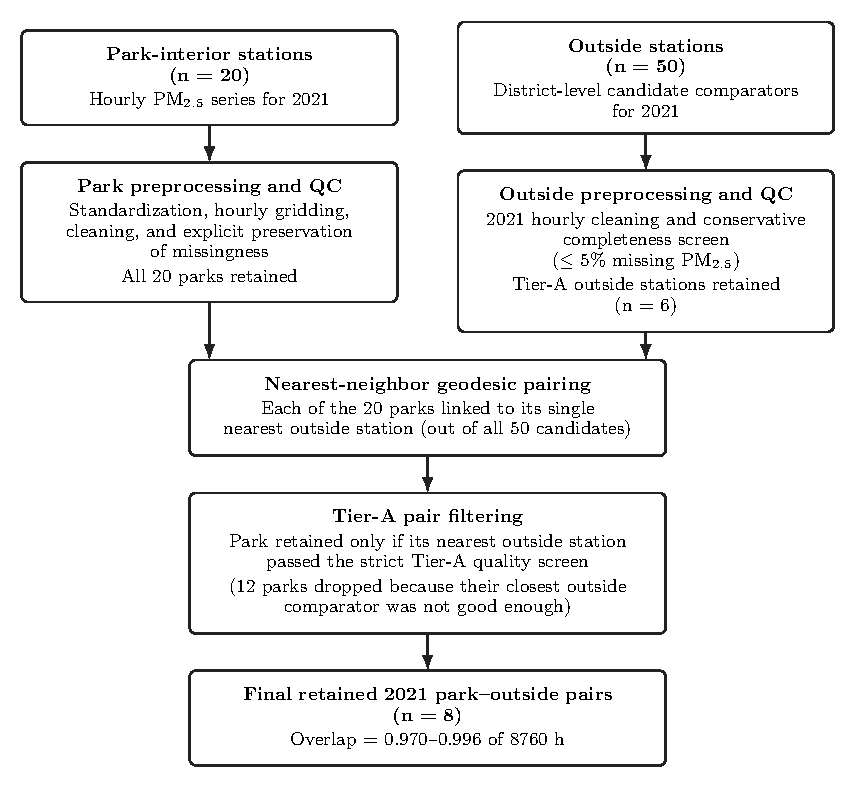
\includegraphics[width=0.92\textwidth]{figures/Fig2_qc_screening_flowchart.pdf}
\caption{Quality-control and pairing workflow for the defensible 2021 Bangkok park--outside wavelet analysis. The study began with 20 park-interior stations and 50 district-level outside stations. Park records were standardized, cleaned, and placed on a fixed 2021 hourly grid; all 20 parks remained available for pairing after this stage. Outside stations were screened more conservatively for the main wavelet analysis, and only stations with no more than 5\% missing PM$_{2.5}$ values in the 2021 hourly record were retained as Tier-A outside comparators. Each park was then linked to its single nearest outside station from among all 50 candidates by geodesic distance; pairs were retained only if the nearest outside station had independently passed the Tier-A quality screen, yielding eight final park--outside pairs with high overlapping annual coverage.}
\label{fig:qc_flowchart}
\end{figure}

\subsection{Wavelet attenuation and coherence framework}

Timescale-specific PM$_{2.5}$ behavior was quantified using a continuous wavelet transform (CWT) framework applied to each paired hourly series. The implementation was carried out in Python using the PyWavelets library (\texttt{pywt.cwt}). For the attenuation analysis, wavelet power was derived using the built-in real Morlet wavelet (\texttt{"morl"}). For the coherence analysis, a complex Morlet wavelet (\texttt{"cmor1.5-1.0"}) was used so that the cross-wavelet product and coherence surface were computed from complex-valued coefficients. Target periods were defined on an hourly grid from 2 h to 14 d, and scales were obtained by converting period in samples to wavelet scale using the PyWavelets central frequency for the corresponding wavelet family. The purpose was to decompose the park and outside records into comparable temporal bands so that attenuation and coherence could be evaluated as functions of timescale rather than as single time-averaged differences.

Wavelet attenuation was defined from the ratio of inside to outside wavelet power:
\[
\mathrm{Attenuation\ (dB)} = 10 \log_{10}\left(\frac{P_{\mathrm{in}}}{P_{\mathrm{out}}}\right),
\]
where $P_{\mathrm{in}}$ and $P_{\mathrm{out}}$ denote the park-interior and outside wavelet power, respectively. Negative values indicate damping of PM$_{2.5}$ variability inside the park relative to the outside comparator, whereas positive values would indicate amplification. The analysis window covered periods from 2 h to 14 d. In the main analysis, a fixed 24-h boundary trim was applied before wavelet summarization to reduce edge effects. Because a fixed trim does not fully remove long-period cone-of-influence exposure, an additional sensitivity check was performed using a stricter 14-day trim at both ends of the series.

For interpretation, attenuation and coherence were summarized within five predefined period bands, defined exactly in hours as 2--6 h, 6--18 h, 18--30 h (diurnal), 48--168 h (2--7 d), and 168--336 h (7--14 d). These bands were selected to separate short-term fluctuations, sub-diurnal variability, the daily rhythm, and broader multi-day behavior relevant to urban pollution episodes.

For cross-pair summaries, attenuation was reported primarily using the median across the eight retained pairs in order to reduce sensitivity to extreme park-level values, whereas coherence was summarized using the mean because it is bounded between 0 and 1 and showed less extreme dispersion across pairs. This difference in summary metric was adopted to preserve robustness for attenuation while retaining straightforward interpretability for coherence.

Wavelet coherence was used to quantify the degree to which park and outside records remained dynamically coupled at each timescale \citep{Grinsted2004}. Coherence was computed from the complex cross-wavelet product and summarized as a smoothed $R^2(s,t)$ surface, obtained as the squared magnitude of the smoothed cross-wavelet term divided by the product of the smoothed individual wavelet-power terms. Smoothing was implemented as a separable moving-average operation with reflect padding to preserve matrix size, using a 24-h window along the time axis and a 3-bin window along the scale axis. The resulting coherence values were bounded to the interval $[0,1]$ before band averaging. No formal significance test was applied, so the coherence analysis is interpreted descriptively rather than as a significance-thresholded detection framework. High coherence indicates that the park and outside station share similar temporal organization at a given band, even if their amplitudes differ, whereas lower coherence suggests temporal decoupling.

Together, attenuation and coherence provide a more informative paired framework than mean concentration comparison alone. A park may reduce the amplitude of PM$_{2.5}$ variability while still preserving the timing of broader urban oscillations, or it may both damp and decouple from the outside signal. This joint interpretation forms the basis for the regime classification developed later in the Results and Discussion sections.

The overall wavelet-analysis workflow used to derive attenuation and coherence metrics is summarized in Fig.~\ref{fig:wavelet_framework}.

\begin{figure}[htbp]
\centering
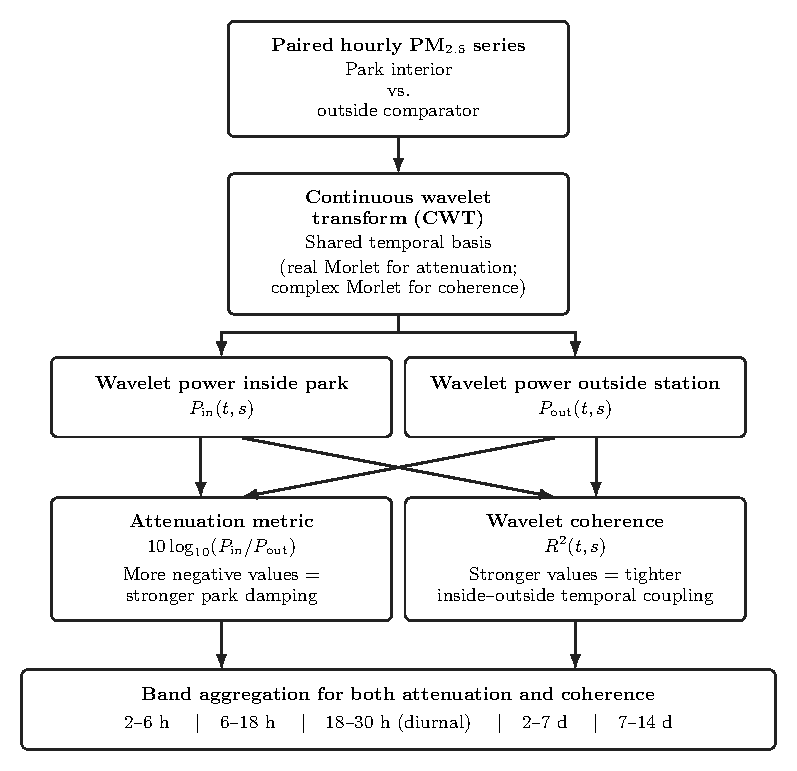
\includegraphics[width=\textwidth]{figures/Fig3_wavelet_framework_schematic.pdf}
\caption{Conceptual wavelet-analysis workflow used for paired 2021 park--outside PM$_{2.5}$ series. Hourly PM$_{2.5}$ records from each park-interior station and its paired outside comparator were transformed into the wavelet domain to obtain timescale-resolved power and coherence information. Inside/outside power ratios were converted to attenuation in decibels, while wavelet coherence was used to quantify the strength of temporal coupling between the two series. Both attenuation and coherence were then aggregated into five predefined bands: 2--6 h, 6--18 h, 18--30 h, 2--7 d, and 7--14 d.}
\label{fig:wavelet_framework}
\end{figure}

\subsection{Spatial explanatory features}

To investigate why some parks displayed stronger damping behavior than others, the study used a layered set of explanatory predictors derived from remote sensing and park geometry. The first layer consisted of station-centered Sentinel-2 indices extracted for both park and outside stations. For the 2021 land-cover stage, NDVI and NDBI were derived from the Sentinel-2 Level-2A surface-reflectance product \texttt{COPERNICUS/S2\_SR\_HARMONIZED} \citep{Drusch2012} over the period 2021-01-01 to 2022-01-01. Scenes were filtered to \texttt{CLOUDY\_PIXEL\_PERCENTAGE < 60}, and a conservative Scene Classification Layer (SCL)-based mask was applied to retain classes 4, 5, 6, and 7 before yearly compositing. NDVI was computed from bands B8 and B4 \citep{Tucker1979}, and NDBI from bands B11 and B8 \citep{Zha2003}. A yearly median composite was then formed, and buffer means were extracted at 10 m resolution for 250, 500, and 1000 m station-centered buffers around both park and outside locations. These products were then transformed into paired contrast variables such as $\Delta$NDVI and $\Delta$NDBI, defined as park minus outside values.

The explanatory framework was then extended from simple mean buffers to annulus-based spatial structure. This was motivated by the possibility that PM$_{2.5}$ buffering depends not only on average greenness, but also on how vegetation and built surfaces are organized radially around the station. Annulus-based summaries were therefore used to characterize ring-gradient patterns around both park and outside locations, allowing the analysis to test whether spatial structure outperformed simple mean land-cover indicators.

A water-related explanatory layer was added later using NDWI \citep{McFeeters1996} and MNDWI \citep{Xu2006}, together with related buffer- and annulus-based water-context summaries. These metrics were intended to capture whether nearby water or moisture-related land-cover structure contributed additional explanatory value beyond vegetation and built-up contrast alone. Because this component was developed after the core wavelet stage, it is treated as a strengthening extension to the 2021 explanatory framework rather than as an independent primary dataset.

A final structural layer described park morphology using polygon-based metrics. These morphology variables were intended to capture aspects of park form that are invisible to mean spectral indices, such as size, shape, compactness, and the potential existence of protected interior space. The explanatory analysis was therefore explicitly multi-layered: mean land cover, ring gradients, water context, and morphology were evaluated as complementary rather than competing descriptions of park buffering context.

\subsection{Exploratory association scans and robustness logic}

Associations between explanatory features and wavelet outcomes were evaluated using exploratory rank-based statistics. The main objective was not formal prediction from a large sample, but rather transparent identification of candidate relationships between spatial structure and timescale-specific damping behavior across the eight defensible 2021 pairs.

Spearman correlation was used to scan relationships between explanatory variables and band-specific attenuation or coherence metrics. The scan was expanded across multiple buffers and feature families, and initial interpretation focused on the strongest absolute correlation values rather than on null-hypothesis significance alone. This was necessary because the effective sample size for pair-level inference was small ($n = 8$), making all statistical findings necessarily exploratory.

To reduce the risk that a single park dominated interpretation, a leave-one-out robustness check was applied to the main land-cover relationship scan. Under this approach, each pair was removed in turn and the correlation recomputed, allowing the stability of candidate relationships to be inspected across all eight leave-one-out subsets. This step was included primarily as reviewer-oriented robustness logic rather than as proof of causality.

Additional annual replication screening was conducted for 2022 and 2023 to test whether the 2021 framework could be extended directly across years. Under the same conservative annual completeness logic used to define defensible outside comparators for 2021, the later-year outside series were found to be too sparse and fragmented for defensible annual wavelet replication. The main manuscript is therefore intentionally framed as a rigorous 2021 Bangkok case study rather than a multi-year annual comparison.